\documentclass{article}
\usepackage{amsmath}
\usepackage{setspace}

% for using images
\usepackage[pdftex]{graphicx}

% for caption manipulation
\usepackage{ccaption}

% Change the format of a figure caption
\captionnamefont{\bfseries}
\captiontitlefont{\small\sffamily}
\captiondelim{ --- }
\hangcaption
\renewcommand{\figurename}{Figure.}

% bibliography packages
\usepackage[sort&compress]{natbib}
\citestyle{nature}

% Some info about the document
\author{Eric S. Shamay, Geraldine L. Richmond}
\title{Aqueous Salt and CCl$_4$ Interfaces}

% some formatting tags
\oddsidemargin  0.0in
\evensidemargin 0.0in
\textwidth      6.5in

% for angstrom symbols
\newcommand{\ang}{~$\textrm{\AA}$~}
\newcommand{\angs}{\ang}
\newcommand{\wat}{H$_2$O~}
\newcommand{\ctc}{CCl$_4$~}
\newcommand{\ctcwat}{H$_2$O-\ctc}
\newcommand{\airwat}{H$_2$O-air~}
\newcommand{\cl}{Cl$^-$~}
\newcommand{\nit}{${\text{NO}_3}^-$~}
\newcommand{\sul}{${\text{SO}_4}^{2-}$~}
\newcommand{\nacl}{NaCl~}
\newcommand{\sodnit}{NaNO$_3$~}
\newcommand{\sodsul}{Na$_2$SO$_4$~}
\newcommand{\costheta}{$\cos\theta$~}
\newcommand{\cosphi}{$\cos\phi$~}
\newcommand{\costhetarange}{~$<\cos\theta<$~}
\newcommand{\cosphirange}{~$<\cos\phi<$~}
\newcommand{\cm}{~$cm^{-1}$~}


\begin{document}
\onehalfspacing

%Abstract
\section*{}

The interface formed between an aqueous salt solution and a hydrophobic liquid has been investigated using molecular dynamics simulations. The salt solutions, \nacl, \sodnit, and \sodsul~ have been studied to determine their presence and distribution in the interfacial region, and their effect on interfacial water molecules. Density and orientation profiles reveal the formation of ionic double-layers with widths that vary with the respective anions' surface affinities, and effects on the geometry of interfacial water molecules. The \nit~anion shows enhanced surface concentration above that of the bulk aqueous phase, whereas the \cl~and \sul~anions exhibit similar characteristics as are found for corresponding air-water interfaces. Sum frequency spectra were calculated for the OH-vibrational modes of water to show the effect of the various ions on the hydrogen-bonding network strength of interfacial water. These calculated spectra show good agreement with the conclusions and observations of our recent spectroscopic experimental study, while providing important new detailed insights into interfacial behavior to augment that study.


% Intro
\section{Introduction}

The most important biological and environmental processes depend on the nature of interfacial water molecules and ions. Only in recent years, and through the development of surface-specific experimental\cite{Charreteur2008,Chen2007,Luo2006,McArthur2006} and computational\cite{Schnell2004,Su2005,Wardle2005,Wick2008a} analytical techniques, have we been able to begin understanding this complex environment of interfacial water and ions. The field has moved from simple water systems in vacuum to studying ever more complex ones such as those near hydrophobic surfaces that are responsible for ion transport, liquid-liquid extraction, drug delivery, and environmental remediation. 

The computational studies presented herein have been conducted to augment recent experimental studies that showed how ions affect the interfacial region between an aqueous ionic solution and a hydrophobic liquid.\cite{McFearin2009} Classical molecular dynamics simulations were performed to analyze the interface formed between various aqueous salt solutions and \ctc. Three salt solutions were simulated, as well as a reference system consisting of neat-\wat for comparison to previous computational efforts.\cite{Hore2007,Hore2008,Hore2007a,Walker2006b,Walker2007a,Walker2007b} The salts used in the simulations were NaCl, NaNO$_3$, and Na$_2$SO$_4$. These were chosen for comparison to the recent experimental sum frequency generation (SFG) spectroscopy results for the same systems,\cite{McFearin2009} and to supplement those experiments with additional molecular-level information. Analyses were performed on the simulation data to extract ionic and molecular density data across organic interfaces, information about water orientation near the interfaces, and simulated SFG spectra. 

%The analyses are similar to, and logical extensions of previous computational work done on aqueous salt systems.\cite{Hore2008,Hore2007a,Hore2007,Wick2006c,Wick2007a,Wick2008,Walker2008}

The computational simulation results provide a microscopic molecular picture of the geometries and interactions occurring within these interfaces that is otherwise inaccessible with experimental methods. The results are in excellent agreement with those of the experimental study, while going further to provide a detailed picture of how water near the hydrophobic liquid surface is altered by the presence of different electrolyte ions, in the aqueous solution, that migrate into the interfacial region. Insights gained from these studies have important implications for understanding a host of environmental, biological, and technological processes involving water near hydrophobic surfaces.

%The results strongly support the experimental study, and provide the first molecular-level look at these water systems at a \ctc interface. Our work builds on years of studies aimed at understanding water's molecular behavior at various interfaces. This work confirms theoretically many of the conclusions we made from experiment, and also provides further microscopic information about aqueous salt systems.



% Overview/methods
\subsection{Density Profiles}

Density histograms of simulated interfaces have been used in previous publications to show ionic and molecular distribution behavior in various systems.\cite{Chang1995,Eggimann2008,Du2008,Wick2006c,Petersen2005a,Hore2008,Walker2006b,Walker2007b} In this work the density profile of water throughout the interface is fit to a hyperbolic tangent function\cite{Wick2006c,MATSUMOTO1988} as shown here:

\begin{equation}\label{tanh_fit}
	\rho(z) = \frac12(\rho_1+\rho_2) - \frac12\left(\rho_1-\rho_2\right)\tanh\left(\frac{z-z_0}{d}\right)
\end{equation}

Equation (\ref{tanh_fit}) relates the interfacial density, $\rho$, as a function of position, $z$, along a given system reference axis, to the densities of the phases, $\rho_1$ and $\rho_2$, on either side of the Gibb's dividing surface (GDS), $z_0$. The interfacial width, $d$, is related to the ``90-10'' thickness that is often reported by $t_{90-10} = 2.197d$.

These measures of interfacial thickness provide a means of comparing the depths to which the water phase is affected by ions located at the interface. The density distributions of the salts depict concentration and depletion phenomena throughout the interfacial region, and also serve to illustrate ionic surface affinity within this region. Previous work has been performed on the \airwat interface with ions of different levels of interfacial affinity, with the more polar ions being the most interfacially active.\cite{Luo2006,Petersen2006,Petersen2005a,Allen2009,Hofft2006,Beattie2005,Bian2009,Dang2004b} We present the density distribution results for the neat \ctcwat and salt solutions adjacent to an organic CCl$_4$ phase. %The density profiles of the different ionic species are fitted using a modified $\tanh()$ function that includes a Gaussian function to more closely fit the concentration near the interface. The anion fitting function allows for a more direct comparison of location and peak width between the different systems.

%\begin{equation}\label{ion_fit}
	%\rho(z) = \frac12(\rho_1+\rho_2) - \frac12\left(\rho_1-\rho_2\right)\tanh\left(\frac{z-z_0}{d}\right) + ae^{-\frac{(x-b)^2}{2c^2}}
%\end{equation}

%The Gaussian function allows one to locate the anion peak height $a$, centered at an offset location $b$, with a width $c$.

%\subsection{Water Coordination}
%The coordination of water and distribution of the various coordination types was determined for each interfacial system. Water coordination refers to the hydrogen-bonding structure of water molecules, and is a measure of the number and type of bonds made. A simple naming scheme used to describe each type of water coordination has been developed previously,\cite{Walker2006b} and so that nomenclature will be used in this work. It has been established that certain bonding structures dominate in different regions of the interface, thus each of the water density profiles will be broken down further into component coordination types to show the areas in which the various types are most prevalent. The parameters used to define a hydrogen-bond are taken from a previous work by this group.\cite{Walker2006b} Analysis of water coordination profiles is valuable for comparison to experimental VSF results within the OH-bond stretching region of the vibrational spectrum. These give a molecular-level description of the composition of an interface, and show the various water bonding types that will contribute most to the VSF signal. Additionally, the results of this work are compared to previous studies on the air and salt water interfaces to establish differences due to the addition of the CCl$_4$ organic phase.

%\subsection{Order Parameters}
%One means of describing molecular orientation near to interfaces is by use of orientational order parameters.\cite{Buffeteau2004} This technique has been applied to biaxial molecules such as water at organic interfaces,\cite{Hore2008} and organic molecules to elucidate structuring within the interfacial region.\cite{Hore2007} In this work we compute the two order parameters, S$_1$ and S$_2$, as functions of distance from the Gibbs dividing surface.

%\begin{equation}\label{s1 parameter}
	%S_1 = \frac12\left<3 \cos^2(\theta) - 1\right>
%\end{equation}
%
%\begin{equation}\label{s2 parameter}
	%S_2 = \frac{\left<\sin(\theta)\cos(2\phi)\right>}{\left<\sin(\theta)\right>}
%\end{equation}

%The order parameters are calculated from the Euler angle values of the molecular ``tilt'' $\theta$, and the ``twist'' $\phi$. %The order parameter distributions are further broken down to show the values for individual water coordination types for determination of orientational behavior of each.

\subsection{Molecular Orientation}
% Describe method used to find the bisector and normal orientation histograms
Several methods have been used previously to show molecular orientation profiles of water molecules throughout simulated interfacial regions.\cite{Wick2006c,Thomas2007,Wick2008a,Wick2007,Fan2009,Galamba2008,Ishiyama2007,Hore2007,Hore2008} Studies have utilized various internal coordinate definitions and a number of angle definitions, orientational order parameters, and probability distributions to relate molecular, or averaged, orientations. In this work we have chosen to compute the orientation of water using two vectors that intuitively describe the orientation in space, given the locations of the three atoms comprising the molecule. The molecular bisector, a vector that points along the axis of symmetry of the water molecule from the hydrogen-end to the oxygen, provides directional orientation similar to the water molecule's dipole. A second vector, that is referred to here as the molecular normal vector, is established as the vector pointing normal to the plane formed by the three atoms of the water molecule and establishes its planar ``tilt''. Analyzing the angle made between these two vectors and a given space-fixed reference axis (herein defined as the long-axis of the simulation cells, oriented perpendicular to the interfacial plane and pointing out of the aqueous phase) is a means of finding the orientation of waters within these simulated systems as illustrated in Figure \ref{fig:water-angles}. The angle formed between the molecular bisector and the reference axis will hereafter be referred to as $\theta$, and the angle between the reference axis and the molecular normal vector as $\phi$. The analysis in this work reports the cosines of these two angles, and because of the symmetry of the water molecule where the hydrogens are not uniquely identified, the cosines of the two angles are limited as follows: $-1\le\cos\theta\le1$ and $0\le\cos\phi\le1$. We report the orientation profiles of $\theta$ and $\phi$ as functions of the distance from the GDS of the interface, as found from the fitting in our density profile analyses.

\begin{figure}[h!]
\begin{center}
	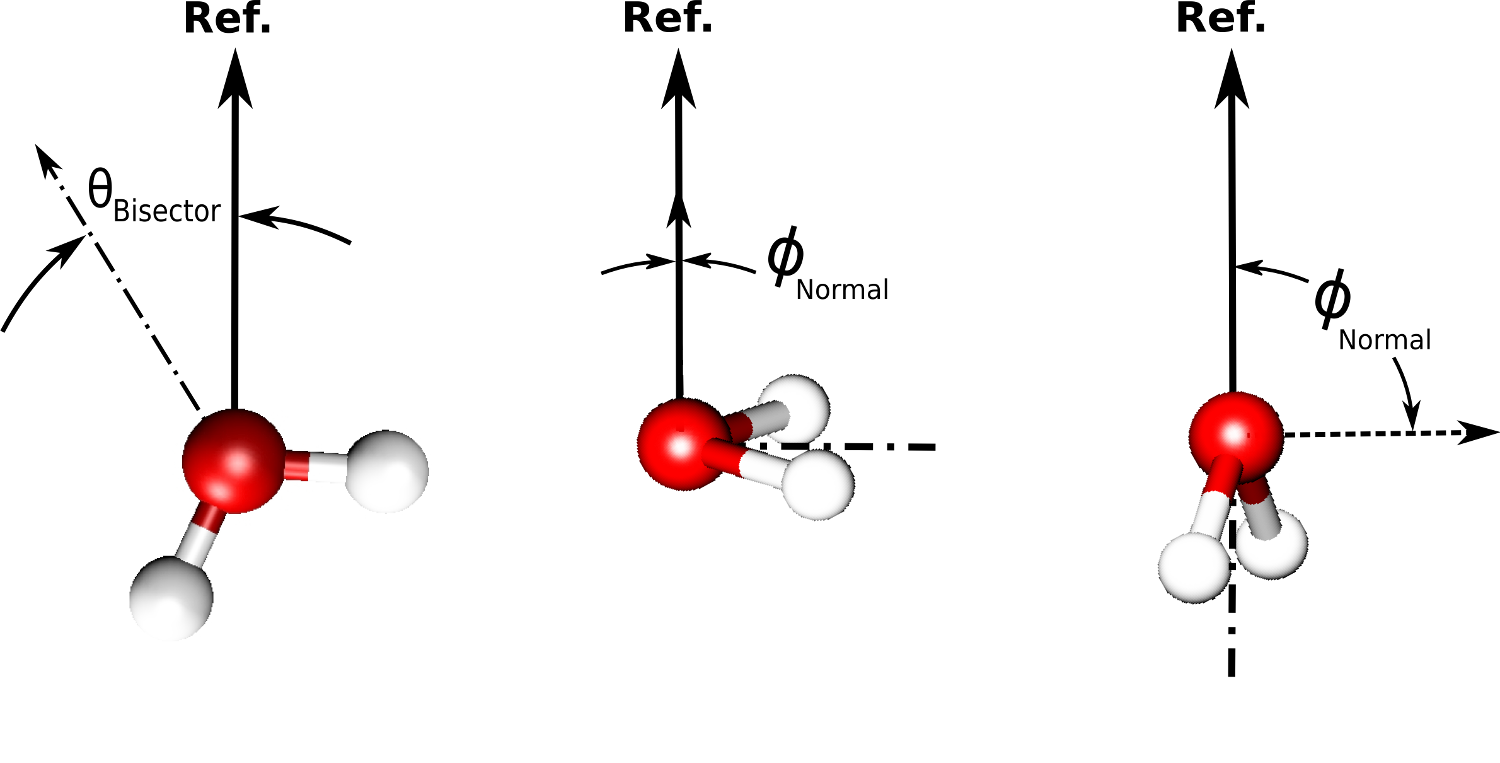
\includegraphics[scale=1.0]{images/water-angles.png}
	\caption{Angles used to define molecular orientation. The system reference (Ref.) axis is that which is perpendicular to the plane of the aqueous-organic interface, and points out from the aqueous phase into the organic one. The molecular bisector vector points from the hydrogen-end of the water to the oxygen end, and orients along the axis of symmetry. The angle it forms with the reference axis is either aligned or anti-aligned such that $-1\le \cos\theta \le 1$. The angle formed between the vector normal to the molecular plane (formed by the three water atoms) and the reference-axis orients the ``twist'' of the molecule such that $0 \le \cos\phi \le 1$, where the water molecular plane is either laying flat on the interface ($\cos\phi=1$), or the water is perpendicular to the interface ($\cos\phi=0$).}
	\label{fig:water-angles}
\end{center}
\end{figure}

%\begin{figure}[h!]
%\begin{center}
%	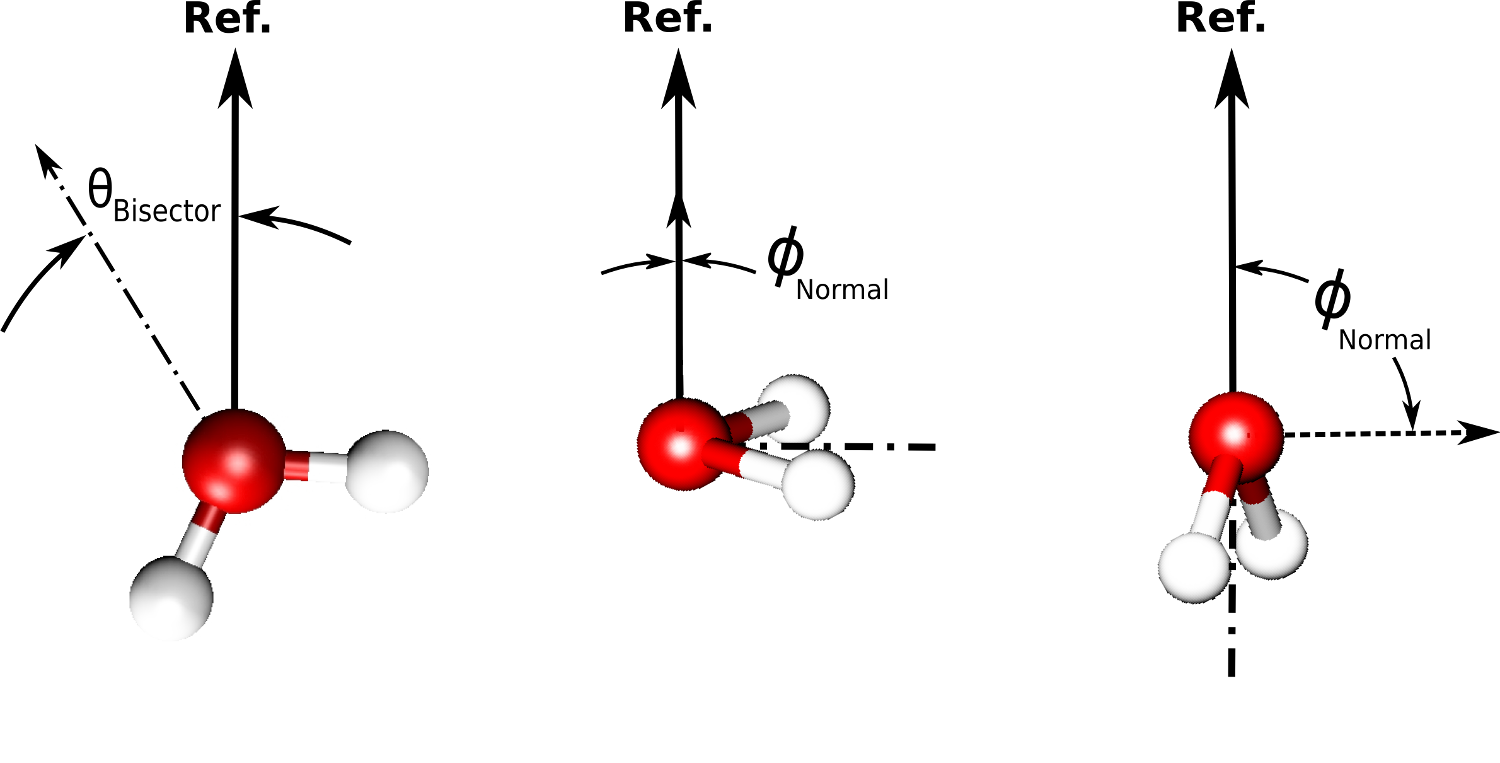
\includegraphics[scale=1.0]{images/water-angles.png}
%	\caption{Molecular orientation of water molecules. The system axis perpendicular to the aqueous interface is used as a reference for analysis of molecular orientation. The angle formed between the reference axis and the water molecular bisector vector, $\theta$, may vary such that $-1<\cos(\theta)<1$. When $\cos(\theta)$ is 1, the molecule's bisector is perfectly aligned with the reference axis, and $\cos(\theta)=-1$ results from a perfect anti-alignment. A second angle, $\phi$, describes the molecular ``twist'' about the bisector. The symmetry of the water molecule limits the range of $\phi$ to $0<cos(\phi)<1$. $\cos(\phi)=0$ results from a water that lies with its molecular plane perpendicular to the plane of the interface, and $\cos(\phi)=1$ describes a water lying perfectly parallel to the plane of the interface.
%	\label{fig:water-angles}
%\end{center}
%\end{figure}


%insert graphic showing bisector and water-plane normal vectors relative to the system Z-axis

%\subsection{Radial Distribution Functions}

%n studying the water structure near to the interface with an organic phase, the radial distribution functions (RDF) for the water atoms were computed lending another metric of water's structure. The RDFs, $g(r)$, for each system were calculated and normalized to a gas-phase probability of unity at long distances, representing a complete loss of orientational correlation.

\subsection{Computational SFG}
%Describe SFG computational method
A difficult challenge for experimental surface studies is in understanding the vibrational spectroscopy of liquid water. Hydrogen bonding between water molecules causes inter- and intramolecular couplings that lead to broad spectral envelopes, each containing a distribution of water-bonded species. Simulations provide the analytical capacity to relate the broad lineshapes, and the often difficultly-assessed impact of hydrogen bonding as a function of OH vibrational frequency, to microscopic geometries, forces, and environments. In this work we compute the SFG spectra of the interface between the salt solutions and an organic phase to compare with the experimental results of similar systems.\cite{McFearin2009} 
%Where general agreement is found, we extract from the calculations a more microscopic picture of the interface and water's spectroscopic signatures to compliment the picture derived from the experiment.

The computational method used in this work is based on that of Morita and Hynes\cite{Morita2000} as outlined in a previous study by this group utilizing the same technique.\cite{Walker2008} The computational SFG technique has been improved in more recent studies by Morita et al,\cite{Morita2002,Ishiyama2009} and with other enhanced water models. The technique used in this work matches qualitatively the experimental spectra to a sufficient degree such that we may draw qualified conclusions about lineshape and intensity. 

%Our present analysis is concerned primarily with the overall intensity and response, and thus we still draw qualitative conclusions based on our computed results, and utilize the simpler computational methods of our previous works.

%The most challenging short-coming of the current technique is that of reproducing accurately the lower-frequency features of the SFG spectra below the 3200\cm region. 

\section{Computational Setup}

The molecular dynamics methods used in this work are similar to those from our previous computational efforts with some modifications described below.\cite{Hore2008,Walker2006b,Hore2007} Simulations were carried out using the Amber 9 software package. The polarizable molecular model parameters are taken from previous works on similar systems.\cite{Chang1997a,Dang1999,Thomas2007,Hrobarik2006,Chang1995} The polarizable POL3 model was used for water molecules.\cite{Caldwell1995} Fully polarizable models have been used in previous interface simulation studies because they are known to more accurately reproduce interfacial structure and free energy profiles.\cite{Rivera2006,Wick2007,Petersen2005b,Dang1998}

A total of 4 systems were simulated consisting of aqueous salt and CCl$_4$ phases. A slab geometry was used to produce two interface regions, the analyses of which were averaged.\cite{Hore2007} The organic region was formed in a box 30-\ang\ on a side with 169 CCl$_4$ molecules to reproduce standard temperature density of 1.59-$\frac{g}{mL}$. The aqueous region was formed in a box 30x30x60-\ang, with the long axis labeled the $z$-axis. The number of water molecules and ions varied for each system in order to reproduce a density of 1.2-M. The specific populations of each molecule are listed in table \ref{densities}. The organic and aqueous boxes were then joined to form a system 90-\ang\ long with interface areas of 30x30-\ang.

\begin{table}[htdp]
	\begin{center}
	\begin{tabular}{|c||c|c|c|}
		\hline
		System & H$_2$O & Cation & Anion \\ \hline
		Neat Water & 1800 & 0 & 0 \\ 
		NaCl & 1759 & 40 & 40 \\
		NaNO$_3$ & 1732 & 40 & 40 \\
		Na$_2$SO$_4$ & 1740 & 86 & 43 \\
		\hline
	\end{tabular}
	\end{center}
	\label{densities}
	\caption{Aqueous molecule and ion numbers. Listed are the populations of each component for the 4 simulated aqueous phases. All systems were simulated at near 1.2-M salt concentrations.}
\end{table}

The water, salts, and CCl$_4$ were each randomly packed into their respective boxes with a minimum packing distance of 2.4-\ang. After joining the aqueous and organic phases and forming the two interfaces, the total system was energy minimized using a conjugate gradient method. Following minimization, the system was equilibrated at a constant temperature of 298-K with weak coupling to a heat bath for a period of 10-ns, using a simulation timestep of 1.0-fs. A non-bonded potential cutoff of 9.0-\ang\ was used. Following equilibration the system was simulated with the same parameters for a further 10-ns with atomic position data recorded every 50-fs. This resulted in a total of 200,000 snapshots which were used in the data analysis.


% Results
\section{Component Densities}

\begin{figure}[h!]
\begin{center}
	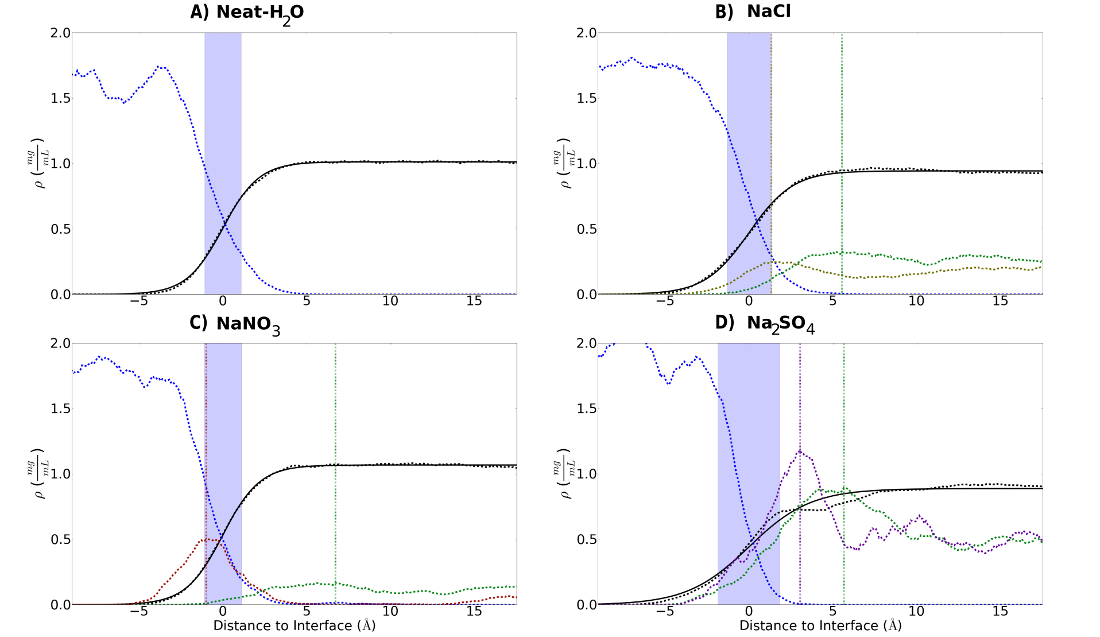
\includegraphics[scale=1.0]{images/densities.png}
	\caption{Aqueous salt solution (1.2 M) and CCl$_4$ surface density profiles. (A) Neat-\ctcwat, (B) NaCl, (C) NaNO$_3$, and (D) Na$_2$SO$_4$ aqueous solution densities are plotted with the water-oxygen density (dashed black) and the corresponding fitted lineshape (solid black). The CCl$_4$ (dashed blue), Na$^+$ cation (dashed green, scaled 10x) and respective anion (scaled 5x) densities are also shown for each system. The maxima of the ionic components are marked with dashed vertical lines of the same colors.}
	\label{fig:density-plots}
\end{center}
\end{figure}

The component density profiles of each system were calculated to study the effects of added salts on water's density profile, and to find any deviations in the behavior of water from the \ctcwat system. The water density profile of each system was fitted to a hyperbolic tangent function (Eq. \ref{tanh_fit}). The resulting plots are shown in Figure \ref{fig:density-plots}. The profiles were centered about the GDS locations, $z_0$, at 0.0\angs, and all lineshapes are plotted as distances to the GDS. Each interfacial width, $d$, is designated as a highlighted blue region of width $d$ centered about $z_0$. The widths of the interfacial regions for the neat-\ctcwat (A), NaCl (B), NaNO$_3$ (C), and Na$_2$SO$_4$ (D) systems are 2.16, 2.62, 2.20, 3.69\angs, respectively. In each of the salt solutions, the anion density profile shows higher density near the interface, appearing as a peak in the density profile. These anion enhancements all occur closer to the interface than the corresponding counter-cation density enhancement. Various parameters of interest such as the interfacial thicknesses, ionic enhancement locations (taken to be the location of the maxima in the ion profiles), and relative distances between the peaks of the ion profiles are collected in Table \ref{table:double-layer}.

\begin{table}[htdp]
	\begin{center}
	\begin{tabular}{|c||c|c|c|c|}
		\hline
		System & $d$ & Anion & Cation & Anion-Cation Distance \\ \hline
		Neat-H$_2$O & 2.16 & - & - & - \\ 
		NaCl & 2.62 & 1.33 & 5.53 & 4.20 \\
		NaNO$_3$ & 2.20 & -0.99 & 6.71 & 7.70 \\
		Na$_2$SO$_4$ & 3.69 & 3.04 & 5.64 & 2.60 \\
		\hline
	\end{tabular}
	\end{center}
	\caption{Aqueous salt system density parameters. Interfacial widths, $d$, and the locations of the maxima of the density profiles for each ionic component are listed for the simulated salt systems. The relative distances between the anion and cation density peak locations are listed to show how the different anions affect the relative location of their cationic counter-ions.}
	\label{table:double-layer}
\end{table}

The oscillations in the surface density profiles of water and the adjoining organic \ctc liquid phase have been noted previously and attributed to thermal capillary waves on a larger length-scale than the simulated system size.\cite{Chang1996} The same work also made note that the interfacial thickness is size-dependent on the interfacial surface area. Increasing the surface area dimensions should therefor cause a proportional increase in the interfacial width. As a consequence, care must be taken when making quantitative comparisons between widths and locations found in differing simulation studies. However, relative width ordering between similarly-sized systems should remain, as shown in two separate works on the \ctcwat surface.\cite{Chang1996,Hore2008}

In comparing the three salt solutions studied here, any differences in these systems are the result of the anion because the same cation was used in each system. \nacl is the simplest of the three salts with a monatomic and monovalent anion. The peak of the anion density profile is within the aqueous phase (i.e. it is found on the aqueous-side of the interfacial width). The location of the cation density peak is, as mentioned above, deeper into the aqueous phase than the anion by over 4\angs. This layering of ions within the aqueous phase is attributed to the break in the isotropy of the field of the bulk region upon introduction of the organic phase. From our studies it is clear that polarizable monovalent anions move towards the interface and effectively screen the induced field from the organic phase. The counter-ions then are drawn towards the negative charge built up by the anions to create the second ion density peak deeper in the aqueous phase. The overall shape of the water profile in the \nacl system is relatively unaffected (compared to the reference \ctcwat system Figure \ref{fig:density-plots}a) by the presence of the ions. The width of the interface is slightly increased above that of the reference system.

%In an MD study by Wick and Dang\cite{Wick2007a} of \ctcwat interfaces, larger and more polarizable monovalent anions exhibited a smaller density enhancement when compared to the \airwat interface. The \ctcwat interface was found to be a less favorable solvation environment for the more polarizable anions. 

%A break in the isotropic environment around the ions causes them to be less solvated and come in greater contact with the \ctc phase. The ions are thus pushed further into the aqueous bulk and more hydrated than at an air-interface. However, the surface activities and ion density enhancements of the more polarizable anions (i.e. I$^-$, Br$^-$) remain greater than that of a smaller and less polarizable one (i.e. Cl$^-$) at both interfaces. 
%Few surface-specific experimental analyses (i.e. SFG) have been performed on these \ctc systems and were mostly limited to the \airwat surface.

It is important to note from our density calculations that ions that increase the interfacial width at the \ctcwat interface correspond to ions that result in an enhancement of the SFG signal from interfacial water. As discussed later, our SFG calculations show excellent agreement with experimental results that also show this enhancement for such ions. Also, we find those ions that are best known to enhance the strength of hydrogen-bonding (i.e. \sul) produce wider interfaces with greater water penetration into the \ctc phase.

The \sodnit system introduces the monovalent, polyatomic nitrate anion. In our simulation we find a strong surface density enhancement of the nitrate anion as shown in Figure \ref{fig:density-plots}(c). The nitrate density peak is located the furthest out from the aqueous phase of the three salt systems. The location of the sodium cation peak in this system is a significant distance further into the bulk water relative to the anion than in either of the \nacl or \sodsul systems. The increase in ion-pair distance is likely the result of strong screening of the interfacial field by the surface-active anion, and the solvating waters around it. The interfacial width of the \sodnit system is the narrowest relative to the other salts in this study. It is likely that slight reorientation of the surface waters near \ctc enhance the solvation of the \nit in the plane of the interface and establish a much more hydrated region for the anion to adsorb. Water reorientation is more fully described later in this work. The subsurface waters then continue to screen the charge of the surface-active \nit, and decrease the coulombic force pulling the cation closer to the surface. 

%Water's ability to extend into the organic phase is affected by its hydrogen-bond network strength. Nitrate acting to break the surface water bonding thus decreases the width of the water penetration into the organic phase. 

The widest interface is that of the \sodsul solution, indicating that the \sul anions act to increase the number of interfacial water molecules on both sides of the GDS, consistent with the highly solvated nature of \sul and its larger size. \sul density enhancement (the peak of the anion density profile) is furthest into the aqueous bulk of the three anions simulated. The calculations suggest that the divalent and highly polarizable nature of the \sul anion attracts its counter-ion closest, leading to the narrowest sub-surface ionic double-layer. This attraction is likely coulombic. Although the greatest anionic concentration enhancement is further into the bulk water region, seemingly outside the region designated by the interfacial width, the water interfacial width is still greatly enhanced. This is in agreement with the experimental \sodsul SFG studies where sulfate ion leads to an enhanced SFG signal throughout the bonded OH stretch region, consistent with a larger interfacial width.\cite{McFearin2009}

%Unlike the monovalent ions, the divalent \sul anion has a very large first solvation shell and prefers a location deeper into the aqueous phase at the \airwat interface,\cite{Salvador2003} and is perhaps repelled from the interfacial region.\cite{Gopalakrishnan2005} This more highly-solvated anionic behavior coincides with the \ctcwat system seen here. Although the presence of the \ctc changes the interfacial environment from that of the \airwat interface, the field established by the deep aqueous-side location of the \sul anion density enhancement acts to affect the interface from a greater distance. 

The results of these and related simulations of ions at liquid-liquid interfaces, and the recent experimental results of similar systems demonstrate that some ions behave at the \ctcwat interface very differently than what has been calculated and observed at air-water interfaces.\cite{Wick2006,Wick2007a,Jungwirth2006a} The most striking example is that of the polyatomic nitrate ion which has been investigated at the \airwat interface by computer simulation,\cite{Miller2009,Thomas2007} spectroscopy,\cite{Otten2007,Schnitzer2000,Xu2009} and depth resolved X-ray photoemission spectroscopy.\cite{Brown2009} In contrast to what is observed here and in the related experimental SFG studies of the \ctcwat interface where nitrate ion shows an enhanced presence in the interfacial region, at the \airwat interface the nitrate ion shows no greater affinity for the surface than the bulk water. The large planar geometry of the \nit anion and its low charge appear to repel it from the \airwat surface where it encounters a reduced solvent cage and seeks a more hydrated solvation state. For \sul ion, experiments at both the \airwat\cite{Gopalakrishnan2005} and \ctcwat interface indicate sulfate does alter the interfacial region, consistent with what is observed in these computations. Unlike the monovalent ions, the divalent sulfate anion has a very large first solvation shell. These calculations indicate that at the \ctcwat interface it prefers a location deeper into the aqueous phase region and affects the interface from a greater distance than the other ions. The comparison of these computations with SFG experimental results will be discussed in more detail later in the paper.

% ********comparison to air-water**********
% Use this paragraph to talk about the differences with the AIR-water systems, and back it up with stuff found from calculations
%The majority of liquid surface studies examining ion behavior over the past decade have been conducted on \airwat interfaces. A recent review elucidates the convergence of data and conclusions regarding \airwat systems, paying special attention to relevant computational efforts.\cite{Jungwirth2006a} Ion behavior at liquid-liquid interfaces, however, is clearly different than these \airwat computational studies. The large polarizable and monovalent anions (\cl, Br$^-$, I$^-$) undergo concentration enhancement above bulk levels at the \airwat interface more than at the organic interface.\cite{Wick2006c,Wick2007a} 

%The behavior of molecular anions such as \nit at \airwat has been explored recently with computer simulation,\cite{Thomas2007,Miller2009} spectroscopy,\cite{Soule2007,Xu2009,Otten2007} and depth-resolved X-ray photoemission spectroscopy.\cite{Brown2009} Studies tend to agree that the \airwat surface affinity of the \nit anion is no greater than the water bulk (i.e. for large simulated systems), but conclusions differ on the extent of density depletion or enhancement. The large planar geometry of the \nit anion and its low charge appear to repel it from the \airwat surface where it encounters a reduced solvent cage, and seeks a more hydrated solvation state. In comparison the \nit does alter the \ctcwat interface with its density greatly enhanced within the surface region above bulk levels. Also, a wide ionic double-layer is established with its counter-ion left deeper in the aqueous bulk. 


%The surface enhancement calculated from MD studies, however, portrays the lower bound of the actual effect because of the reduced polarizability values used in simulations to avoid the so-called ``polarization catastrophe.'' Anionic surface enhancement occurs in both liquid-vapor and liquid-liquid simulations, but the enhancement effect is greater at the air-water interface than at \ctcwat.\cite{Wick2007a} 

%Ionic double-layers at both \airwat and \ctcwat surfaces have been documented in many of the studies already referenced. The distance between the anion and cation subsurface enhancements at the \ctcwat interface are shown in Table \ref{table:double-layer}. In an SFG experiment performed on the \airwat interface, Xu et al\cite{Xu2009} probed the vibrational modes of the \nit anion, rather than water's OH modes finding two anionic surface species. They concluded that solvation from an abundance of water at the interface weakens coulombic forces between ions, leading to greater cation-anion separation. The surface nitrate is dehydrated, and the water provides adequate shielding of the ionic coulombic interactions. We find ion double-layering at the \ctcwat interface with no contact-ion pair formation for each of the salts. Likely, this is due to the stronger reorientation of water in the presence of the organic phase, and the subsequent field-screening by sub-surface waters between the ionic layers.

%Ionic double-layers at both \airwat and \ctcwat surfaces have been documented in many of the studies already referenced. The distance between the anion and cation subsurface enhancements at the \ctcwat interface are shown in Table \ref{table:double-layer}. An SFG study by Schultz et al. using similar sodium salts noted the double-layer at the \airwat interface and attributed it to a ``displacement'' mechanism binding ions to interfacial waters, and forming contact-ion pairs. This was based on the lower-frequency OH vibrational mode found at 3150\cm, and the lack of signal change with added salts. Since then Xu et al studied this phenomena with an SFG experiment finding no ion-pairing in solution of various nitrates with divalent cations at the \airwat interface.\cite{Xu2009} The same study probed the vibrational modes of the \nit anion, rather than water's OH modes finding two anionic surface species. They concluded that solvation from an abundance of water at the interface weakens coulombic forces between ions, leading to greater cation-anion separation. The surface nitrate is dehydrated, and the water provides adequate shielding of the ionic coulombic interactions. We find ion double-layering at the \ctcwat interface with no contact-ion pair formation for each of the salts. Likely, this is due to the stronger reorientation of water in the presence of the organic phase, and the subsequent field-screening by sub-surface waters between the ionic layers.

%As compared to our experiment,\cite{McFearin2009} the \ctcwat double-layer size appears inversely proportional to the SFG signal enhancement of water OH vibrational modes. The tighter ionic double layer of the \sul system produces the greatest enhancement above the neat-\wat spectrum, and the widest double-layer of \nit decreases it markedly.

%It is reasonable to assume that this same effect may cause the greater cation-anion separation at the interface of the \sodnit system, even in the presence of the organic phase.

%Simulations of air-liquid systems have recently converged to a picture of an interface with enhanced ion concentrations for small monovalent ions,\cite{Wick2008a}little or no ionic density enhancement above the bulk levels for .\cite{ Surface-specific SFG has been used to characterize structural changes in the water hydrogen-bonding network at the air interface in the presence of various anions.\cite{Schnitzer2000} It was found that SFG signal from the interfacial waters was affected

%The neat-\airwat system has been simulated and analyzed previously,\cite{Wick2006c,Hore2008,Wick2008a} and is the benchmark for comparison to organic-\wat studies. Deviations in width of the interface from the neat-\ctcwat system can be attributed to the added ions in the solution. One work used SFG to detect structural changes in the water hydrogen-bonding network at the air interface in the presence of various anions, and found that it affects the SFG signal intensity from the interface, but could not create the anion density profile\cite{Schnitzer2000}. The same work found SFG intensity enhancement for hydrogen-bonded water following a trend of H$_2$SO$_4\ge$ HCl $>$ HNO$_3$. Comparison with an \airwat MD study complements this trend finding that the \sul concentration enhancement was found furthest into the water bulk.\cite{Salvador2003} Although the SFG studies stopped short of reporting a concentration profile, a recent X-ray photo-emission spectroscopy study was performed to specifically determine the nitrate concentration profile for the water-vapor interface, and reported the current differences of opinion between experiment and simulation.\cite{Brown2009} The XPS results showed a surface depletion of the nitrate anion relative to the bulk, similar to previous MD simulations of the same systems. Other works performed on the liquid-vapor interface found similar nitrate surface depletions.\cite{Otten2007} These help to contrast the effect of the presence of an organic phase as in the present work. 

% Use this paragraph to talk about the discrepancy between the nitrates at the air-water vs at the ctcwat. Also, add in the reference to the latest tobias/jungwirth/finlayson-pitts.

%Previous simulations found concentrations of small monovalent anions to be lower at the \ctcwat interface than at the air-liquid one.\cite{Wick2007a} Most of the recent studies on ion concentration near water interfaces have noted that large and polarizable ions will concentrate at the air surface,\cite{Petersen2005b,Pegram2006,Sloutskin2007,Eggimann2008} while small non-polarizable ions tend to be repelled. The surface enhancement calculated from those MD studies, however, portrays the lower bound of the actual effect because of the reduced polarizability values used in simulations to avoid the so-called ``polarization catastrophe.'' The enhancement of surface anions is also believed to be the cause of the subsurface cation density increase. The counter-ions are attracted to the concentrations of anions at the surface, which are in turn stabilized by the increased polarization of the water due to the distorted interfacial electric field. The affinity for the surface follows the trend of surface tension increments, $\frac{d\gamma}{dm_2}$, where Na$_2$SO$_4 >$ NaCl $>$ NaNO$_3$.\cite{Pegram2006} This also follows the Hoffmeister series trend for anions found to be the most ``structure-making'', and they are found to be density enhanced further into the interface. Our simulations for this work thus provide an interesting comparison to the \airwat research, and the analysis shows evidence that an organic phase causes changes in behavior of the surface waters.


\section{Water Orientation}

Previous studies have provided a detailed overview of water orientation at the interface with both air and organic phases.\cite{McFearin2009,Hore2008,Fan2009,Wick2006c,Wick2008a} The topmost water layers are highly disrupted because of their contact with the organic phase, and it has been suggested that ordering of both the organic and water molecules would lead to a field across the boundary of the interface.\cite{McFearin2009,Hore2008} This can influence charged species, and the ordering and orientation of the H-bond network. Our recent experimental SFG results suggest that the accumulation of charged ions leads to a field-screening that affects the orientation of waters in the topmost layers. This is complemented by the results of the current study.

\begin{figure}[h!]
\begin{center}
	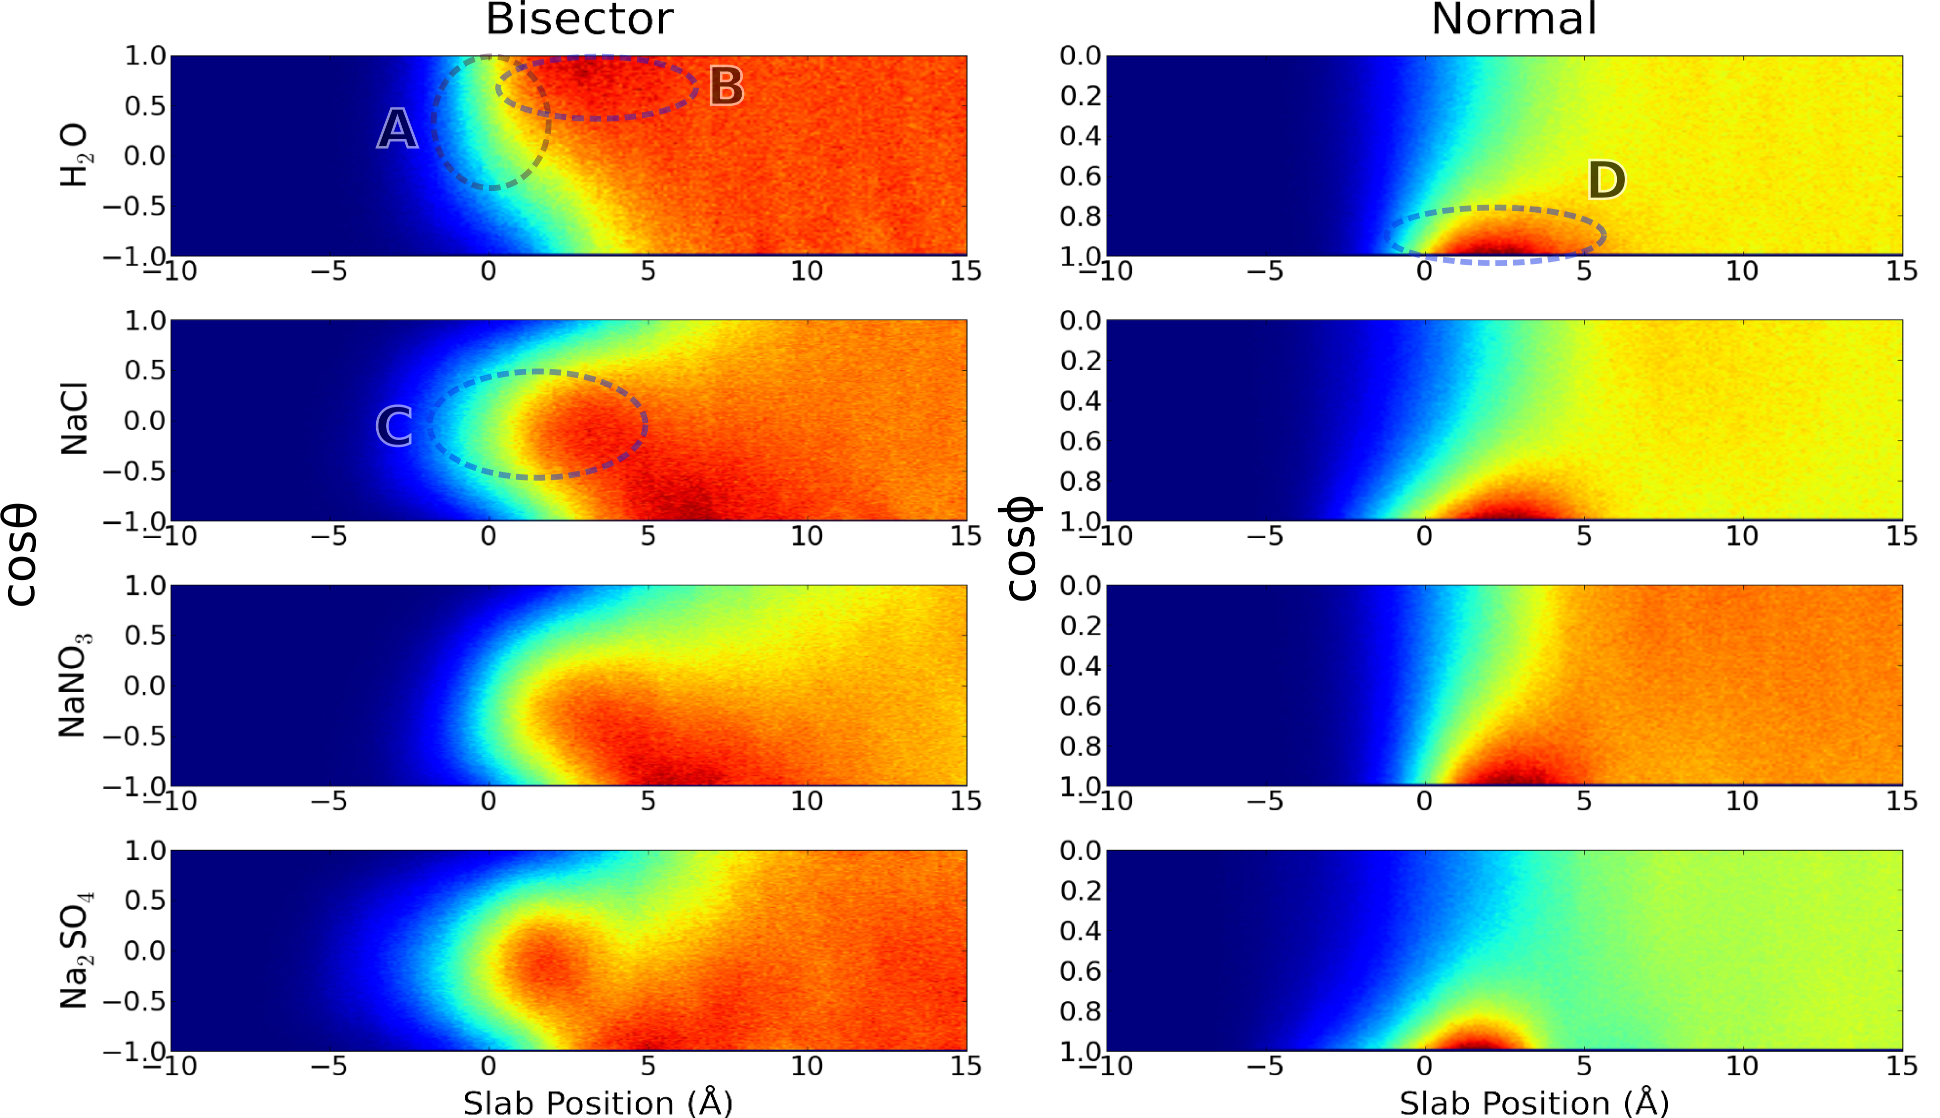
\includegraphics[scale=1.0]{images/h2o-2dhistograms.png}
	%\caption{Orientation profiles of interfacial water molecules. Two profiles were developed for characterizing interfacial water orientation based on the bisector and molecular normal vector angles formed with the system references axis (see Figure \ref{fig:water-angles}). Each profile shows the water population for each cosine of the respective angle as a function of distance to the Gibbs dividing surface (located at 0.0). The profiles in the left column are of the bisector vector, and those on the right are of the molecular normal vector. Neat-H$_2$O, NaCl, NaNO$_3$, and Na$_2$SO$_4$ system profiles are ordered from the top to bottom row, respectively.}
	\caption{Orientation profiles of interfacial water molecules at different depths from the GDS. The molecular bisector profile (left column) and the profile of the molecular axis normal to the plane of the water molecule (right column) are shown. Both angle definitions are depicted in figure \ref{fig:water-angles}, and the angle cosines are plotted here. The neat-\wat, \nacl, \sodnit, and \sodsul system water orientation profiles are plotted from top to bottom row, respectively. Positive position values indicate the aqueous phase, and negative positions are in the \ctc phase. Regions labeled in the profile correspond to orientations depicted in figure \ref{fig:angle-ranges}.}
	\label{fig:2dhisto}
\end{center}
\end{figure}

The orientation of water within the aqueous/organic interface of the system was defined using the angles formed by molecular axes and the fixed reference axis of the system (perpendicular to the interfacial plane). The two molecular axes used are the water bisector, pointing from the hydrogen side to the oxygen, and the vector normal to the plane formed by the three atoms of the water molecule, as depicted in figure \ref{fig:water-angles}. Figure \ref{fig:2dhisto} shows the angle profiles of both the molecular bisector and the molecular plane normal of water molecules relative to the system reference axis at various depths into the aqueous phase. Darker red regions of the plots indicate higher orientational populations, while homogeneous coloring across the angle range indicates orientational isotropy.

\newcommand{\degree}{\ensuremath{^\circ}}

\begin{figure}[h!]
\begin{center}
	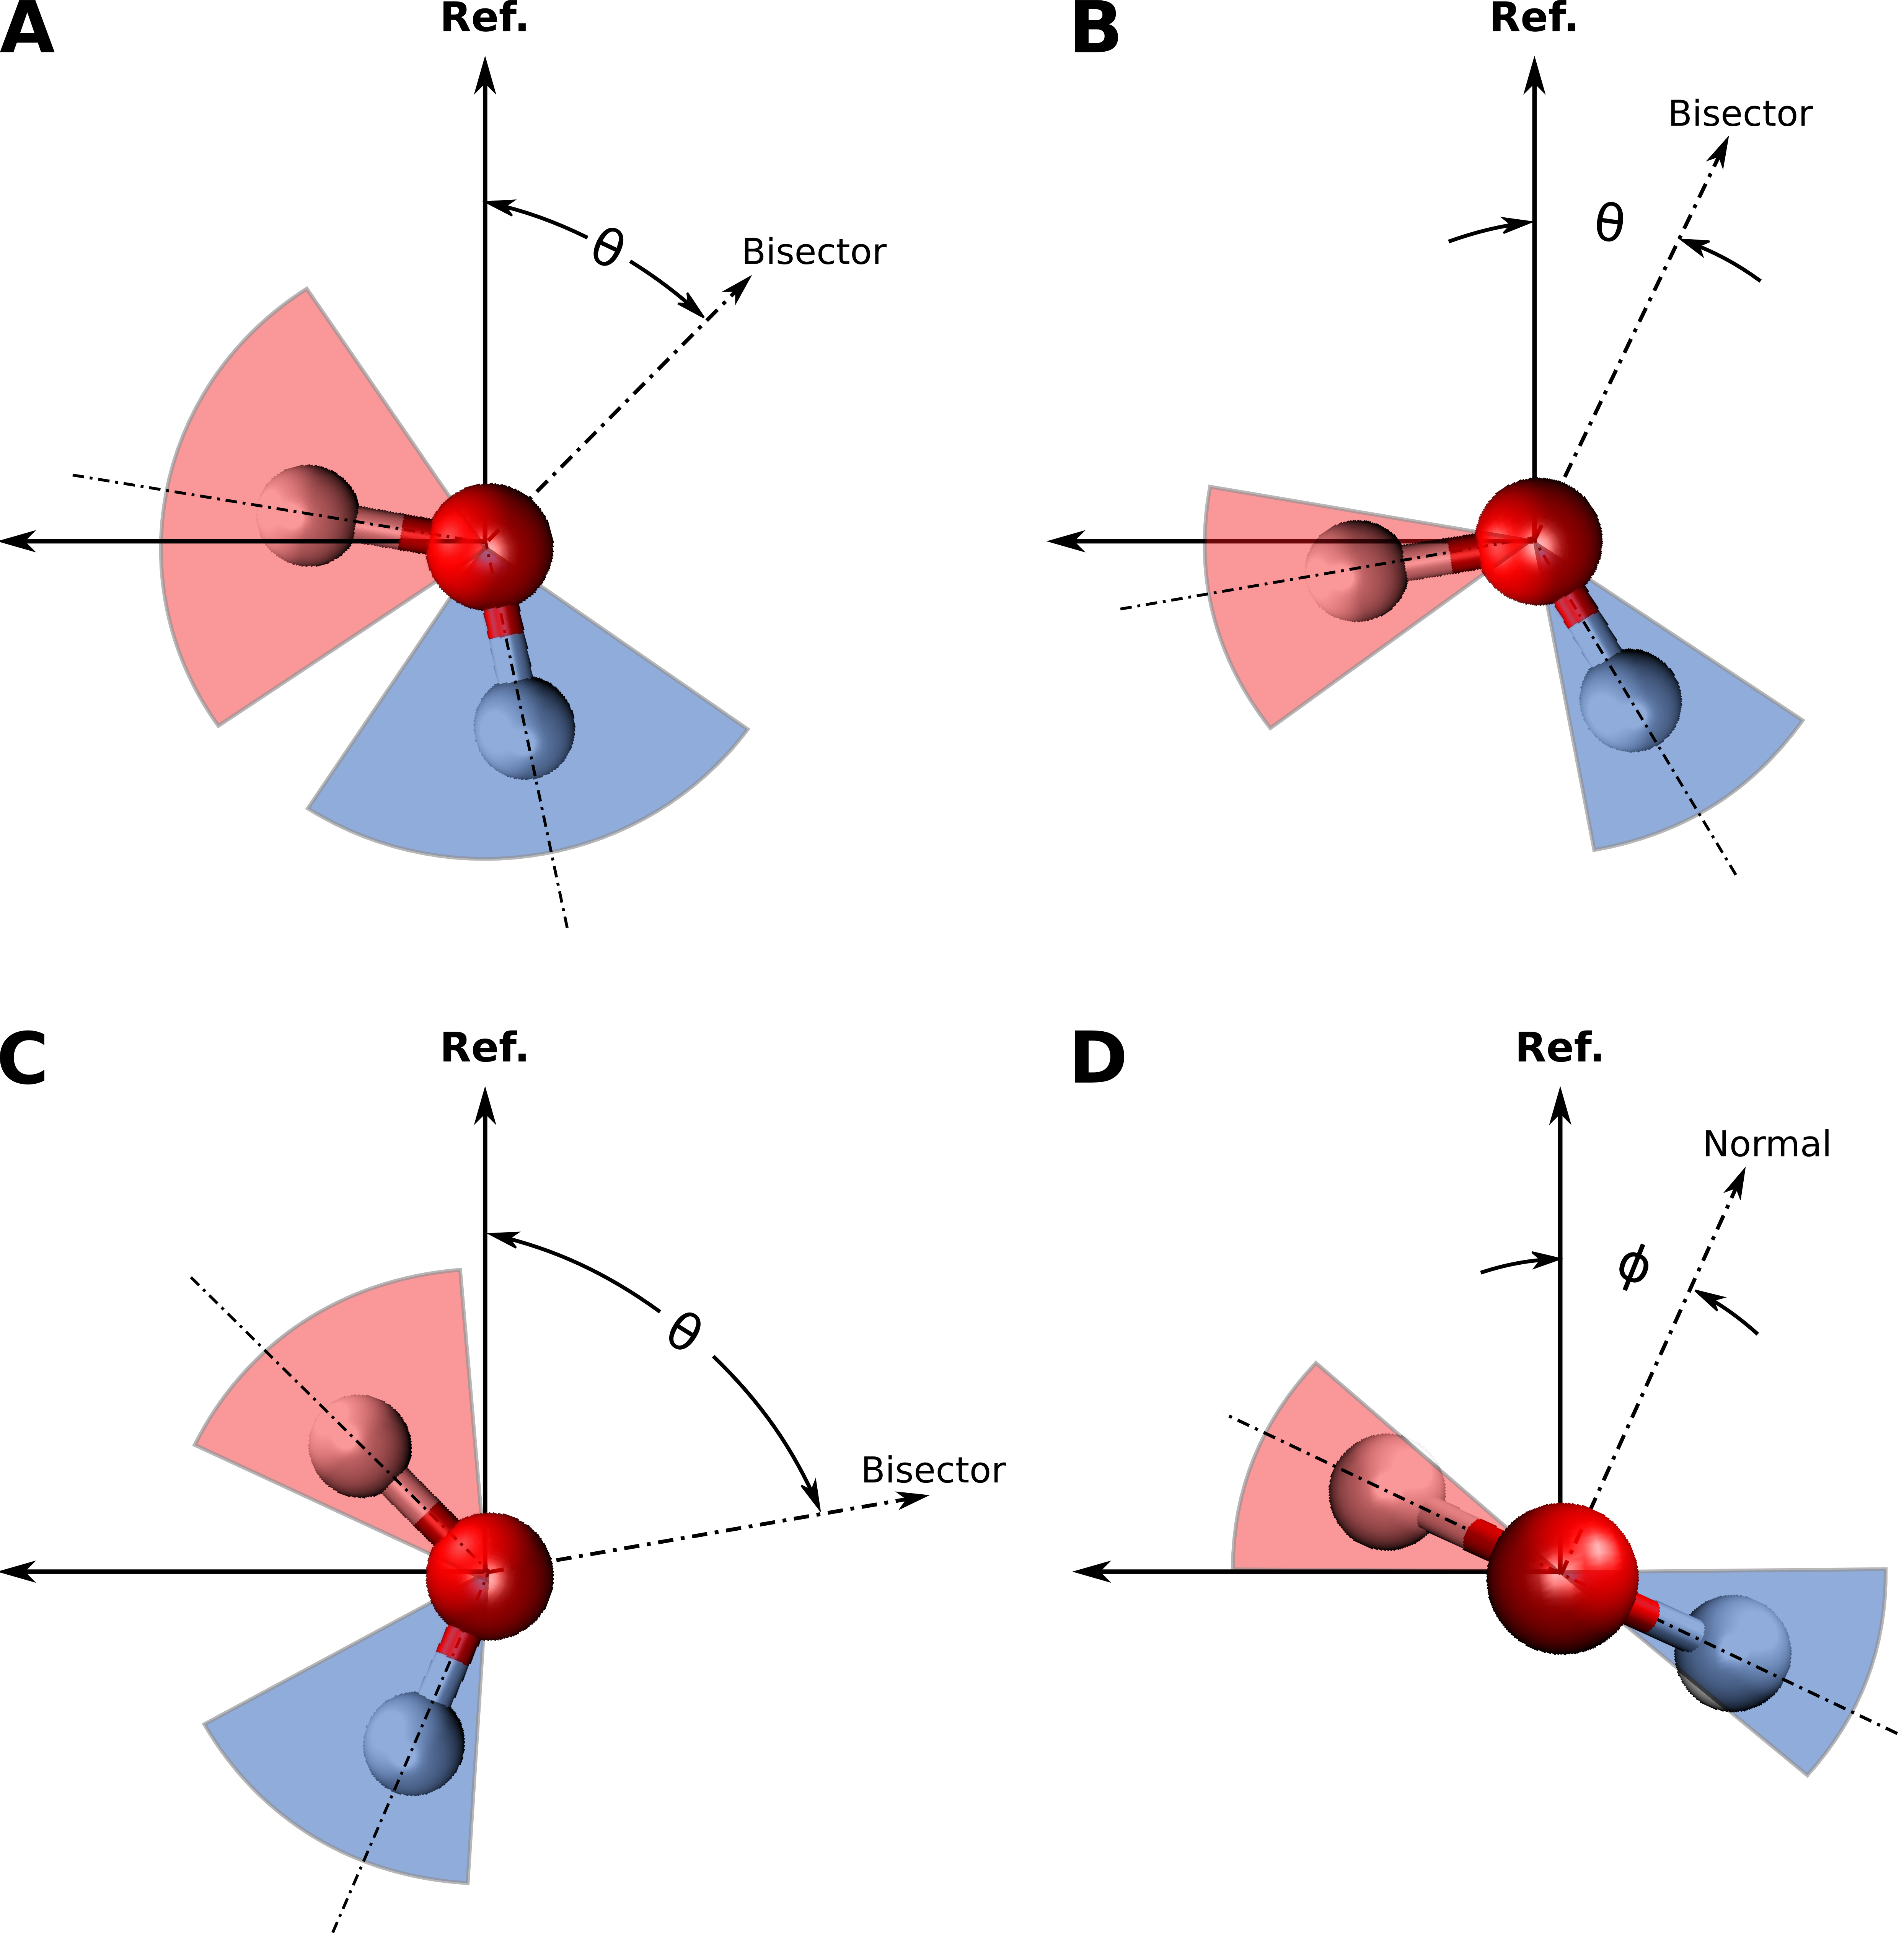
\includegraphics[scale=1.0]{images/h2o-angle-ranges.png}
	%\caption{Depictions of possible orientations for different ranges of the bisector-reference angle $\theta$. A range of 0\costhetarange1 ($0\degree<\theta<90\degree$ - left figure) suggests that one of the OH-bonds will always point into the aqueous phase, and the other will straddle the plane of the interface. In the range -0.5\costhetarange0.5 ($60\degree<\theta<120\degree$ - center figure) one OH-bond will always point out of the aqueous phase, and the other will always remain pointing in towards the water bulk. The molecular normal angle, $\phi$, has a narrow range for interfacial waters in all of the systems spanning approx. 0.7\costhetarange1.0 (right). The range of $\phi$ keeps the topmost waters lying mostly flat on the interface, but with a narrow range of twist with OH-bonds pointing both into, and out of the interface.}
	\caption{Depictions of water orientations ranges spanning varying values of $\theta$ and $\phi$, as defined in figure \ref{fig:water-angles}. The effect of rotating the water within a fixed angle range is illustrated by the shaded (red and blue) regions that bound the OH-bonds. Ranges of $\theta$ shown here are (A) 0\costhetarange1, (B) 0.7\costhetarange1, (C) -0.5\costhetarange0.5. (D) The $\phi$ range of 0.7\cosphirange1 shows the molecular plane of the water mostly flat (i.e. parallel to) the plane perpendicular to the reference axis. Depictions here correspond to those regions labeled in figure \ref{fig:2dhisto}.}
	\label{fig:angle-ranges}
\end{center}
\end{figure}

% Neat-h2o bisector
In the left column of figure \ref{fig:2dhisto} are the bisector orientation profiles for each of the systems. The far-left dark-blue regions of the plots show the \ctc bulk near to the interface where few or no waters are found. The GDS is located at a depth of 0.0\angs. To the far right in the water bulk, the flat, uniformly-colored profile represents the expected isotropic orientation of the waters. The regions of interest lie around the GDS within the interface. The top bisector profile is that of the neat-\wat system, and it shows a transition in the profile beginning a couple\angs into the \ctc phase, and extending up to 5\angs into the aqueous side, at which point the profile becomes orientationally isotropic. At the GDS most of the waters are oriented between 0.0\costhetarange1.0, indicating a range of orientation as depicted in figure \ref{fig:angle-ranges}a. In this range one of the OH-bonds points into the aqueous side, and the other straddles the interfacial plane with a slight affinity towards the organic \ctc phase. Just under the water surface, between 2-4\angs into the neat-\wat phase, a dark-red region spanning approx. 0.7\costhetarange1.0 appears. This narrow orientational range is depicted in figure \ref{fig:angle-ranges}b, and is similar to the waters in the topmost aqueous layer nearer to the GDS, but further limited such that one OH bond points into the \wat side, and one of them only straddling the interfacial plane with a tendency to point into the \wat phase.

The neat-\wat bisector orientational profile is comparable to previous simulations of the same neat-\wat reference system. Using different simulation parameters for the same neat-\wat/\ctc system, Wick and Dang found the free-OH to point slightly into the \ctc phase at the GDS with an angle of \costheta$_{free-OH}\approx 0.4$. This corresponds to \costheta$_{bisector} \approx 0.5$ in the this work's angle definition. Similarly, deeper into the surface the angle profile diminishes such that $\cos(\theta_{free-OH})\approx 0.0$ within 5\angs of the GDS, corresponding to $\cos(\theta_{bisector})\approx 0.8$ in the current scheme. Those results agree with this work's neat-\wat profile, further complementing the experimental SFG conclusions performed on the same systems.\cite{McFearin2009,Scatena2001}

%The bisector exhibits an affinity to point such that 0\costhetarange1. The orientation of the OH-bonds for such an angle range is illustrated in figure \ref{fig:angle-ranges}. In the case of the neat-water reference system, the ``free-OH'' bond is generally pointing out of the aqueous phase, but often points within the plane of the interface. At 3\angs into the neat-water surface, there appears a peak spanning approx. 0.7\costhetarange0.9 that stretches out to just past 5\angs, at which point the profile becomes flat across the values of $\theta$.

% Salt bisectors
Bisector angle profiles for the salt systems show different behavior than that of the reference neat-\wat system. The profiles of the salt systems at the GDS all center about the \costheta$=0$ region, with a range of approx. -0.5\costhetarange0.5. This indicates a straddling water molecule with the orientational range depicted in figure \ref{fig:angle-ranges}c. The water in that range is clearly oriented such that one OH-bond always points out of the aqueous phase into the \ctc, and the other always points in to the water bulk. The OH-bond that would straddle the interface in the neat-water system points out of the interface with a greater angle. This orientation, centered about \costheta$\approx 0$, extends into the water phase up to 3\angs, at which point the profile shifts to the darker region near -1.0\costhetarange0.7. The sub-surface region of the profile between 4-7\angs in each system corresponds to a flip of the water orientation, as referred to in a recent SFG study as a ``flip-flop'' model where water orients to counteract the field of charged species at interfaces.\cite{Nihonyanagi2009} The cation density enhancement in each salt system is within the region of 5-7\angs below the GDS. The waters may be orienting with the negatively charged oxygen end towards those cations, and with the field established by the ion double-layer within the interface. In each of the salt bisector profiles there is a clear depletion of waters oriented towards \costheta$=1$ suggesting that alignment of the bisector with the reference axis is not preferred. The effect is most pronounced in the \sodsul system where the distance between counter-ion density enhancements is smallest, and the transition in the bisector profile is the most abrupt, changing from a profile mostly in the range of -1.0\costhetarange0.5 to isotropic orientation quickly near 8\angs into the aqueous phase. The \sodnit system bisector profile shows the effect furthest into the water bulk, extending almost to 13\angs. Counter-ion density enhancement is most separated in \sodnit, however, and most of the orientational affinity for -1.0\costhetarange0.5 occurs within the first 10\angs of the surface. The bisector profile of the \nacl system is broadest with -1.0\costhetarange0.7 starting near the GDS. Also, orientational isotropy is shallowest in the \nacl system starting near 7\angs into the aqueous phase.

It appears that the field established by the anion-cation pairing within the interface affects the depth to which waters are oriented before the bulk isotropic profile begins. Also, the range of orientations beneath the surface is dependent on the properties of the anion. The weakly polarizable \cl anion does not restrict the orientational range as much as the more polarizable \nit and \sul. Anions also appear to control the depth to which the water orientation is felt, with the most surface-active \nit anion causing the deepest effect. \sul anion shows the strongest restriction on the range of bisector angles, and the sharpest orientational transition to the bulk, which may be attributed to the higher charge of the anion, and thus the stronger field established between the counter-ions in the system.

%The sharpest transition in the bisector profiles is that of the Na$_2$SO$_4$ system. This can be attributed to the proximity of the anion and cation density peaks in the water bulk, which is shortest in the system. Following the trend is the broadest bisector profile of NaNO$_3$ that extends past 10\angs past the interface, and corresponds to the greatest anion-cation density peak distance. NaCl follows the trend as the bisector orientation profile extends to the same depth as the Na$_2$SO$_4$ system, but the transition to the isotropic region is not nearly as sharp, as the electric double-layer set up by the anion and cation densities is not as strong. This is both because of the proximity of the ions, but also because of the higher charge of the divalent SO$_4^{2-}$ anion compared to the monovalent Cl$^-$. The field created by the anion-cation pairing within the interface affects both the depth to which waters are oriented, and also the width of the transition to isotropic orientation.

% Water normal
%The molecular plane normal in the right column of figure \ref{fig:2dhisto} is centered about the flatter orientations with 0.7\costhetarange1.0. This profile suggests that the water lies flat on the interface with a twist of up to 45\degree.  Molecular normal orientation profiles are very similar across the systems investigated, with each profile showing an affinity for the flat orientation starting just before the GDS, and extending as deep as 7\angs in the water and \nacl systems, and between 3-4\angs in the \sodnit and \sodsul polyatomic salt systems.

\newcommand{\phiprof}{$\phi$-profile~}

Orientational profiles for the molecular plane normal of the water molecules ($\phi$-profiles) are found in the right-column of figure \ref{fig:2dhisto}. The range of a \phiprof is limited to 0.0\cosphirange1.0 because of the inherent symmetry of the plane of the water molecule. More similarity is shared between the $\phi$-profiles than the bisector profiles for the different systems. The neat-\wat profile is typical of the four profiles in appearance with a large clustering of water population in the range of 0.7\cosphirange1.0 between the GDS and up to 7\angs into the aqueous phase. This particular $\phi$ range is depicted in figure \ref{fig:angle-ranges}d, showing the mostly flat (i.e. parallel to the interface) orientation of the molecular plane. It is notable that the $\phi$-orientation is affected to the same depth as the first peak (dark-red region) of the bisector profile. However, in the salt systems the second peak near to \costheta$=-1.0$ begin at a depth where the \phiprof has already become isotropic. Thus, in the salt systems, the first water layer (between the GDS and almost 4\angs into the surface) has a defined $\phi$-orientation that is rather flat on the interfacial plane, but the deeper waters (4-7\angs into the interface) are isotropic in $\phi$, and oriented with \costheta closer to -1.0 (an orientation with oxygen pointing into the water bulk, and hydrogens more towards the interface).

By virtue of the interdependence of $\theta$ and $\phi$ (the bisector is perpendicular to the molecular plane normal at all times) a value of \cosphi$=1.0$ implies \costheta$=0$, and vice-versa. However, a broad $\theta$-range allows for a full range of $\phi$ values. Although the second peak of the salt-system bisector profiles is concentrated near to \costheta$=-1.0$, the corresponding \phiprof is isotropic. This deeper region (the second water layer) orients with the bisector counteracting the field of the anion-cation double-layer, and the only apparent affinity is that of placing oxygen closer to the cation density enhancement (and hydrogen closer to the anion layer), while the \phiprof spans the entire orientational range.


%\section{Water Orientational Order Parameters}

\section{Calculated Sum-Frequency Spectra}

%One of the aims of this simulation study is to provide complementary information to the SFG experimental studies of these systems.\cite{McFearin2009}
The effect of the varied set of anions on the \ctcwat interface is linked from simulation to empirical data through the computed SFG spectra. The computed spectra for the SSP polarization (polarization schemes are fully described in literature\cite{Lambert2005}) are presented in Figure \ref{fig:sfg-spectra} along with the experimental spectra (inserts) from our previous experimental SFG work with these same salt solutions interfaced with \ctc.\cite{McFearin2009} Each of the spectra show a salt system response (colored traces) overlayed on the reference \ctcwat spectrum (black or dashed-black traces). On first look, the overall computed intensities and lineshapes follow remarkably similar trends as in the experimental systems. All the spectra have a strong feature near 3660\cm coinciding with the ``free-OH'' vibrations as defined previously,\cite{McFearin2009} and corresponding to one of the uncoupled OH stretch modes from water molecules that ``straddle'' the interface (Figure \ref{fig:water-angles} a, b, and c).\cite{McFearin2009} The broad spectral region from 3200-3500\cm is attributed to the more highly-coordinated OH-oscillators that are solvated at the surface, or just beneath the surface with stronger hydrogen-bonding. Each of the spectra computed for the salt-solutions differ markedly from each other and from the neat \ctcwat spectrum. The monovalent ions (\cl and \nit) in solution produce a measurable decrease in intensity of the lower-frequencies of the spectra with very little change to the free-OH mode. Like the experimental counterparts, the decrease is greatest around the 3200-3400\cm region but shows little change from the neat \ctcwat system above 3500\cm. As in the SFG experiment, the presence of the \sul anion causes an opposite effect by significantly enhancing the intensity below 3600\cm.

\begin{figure}[h!]
\begin{center}
	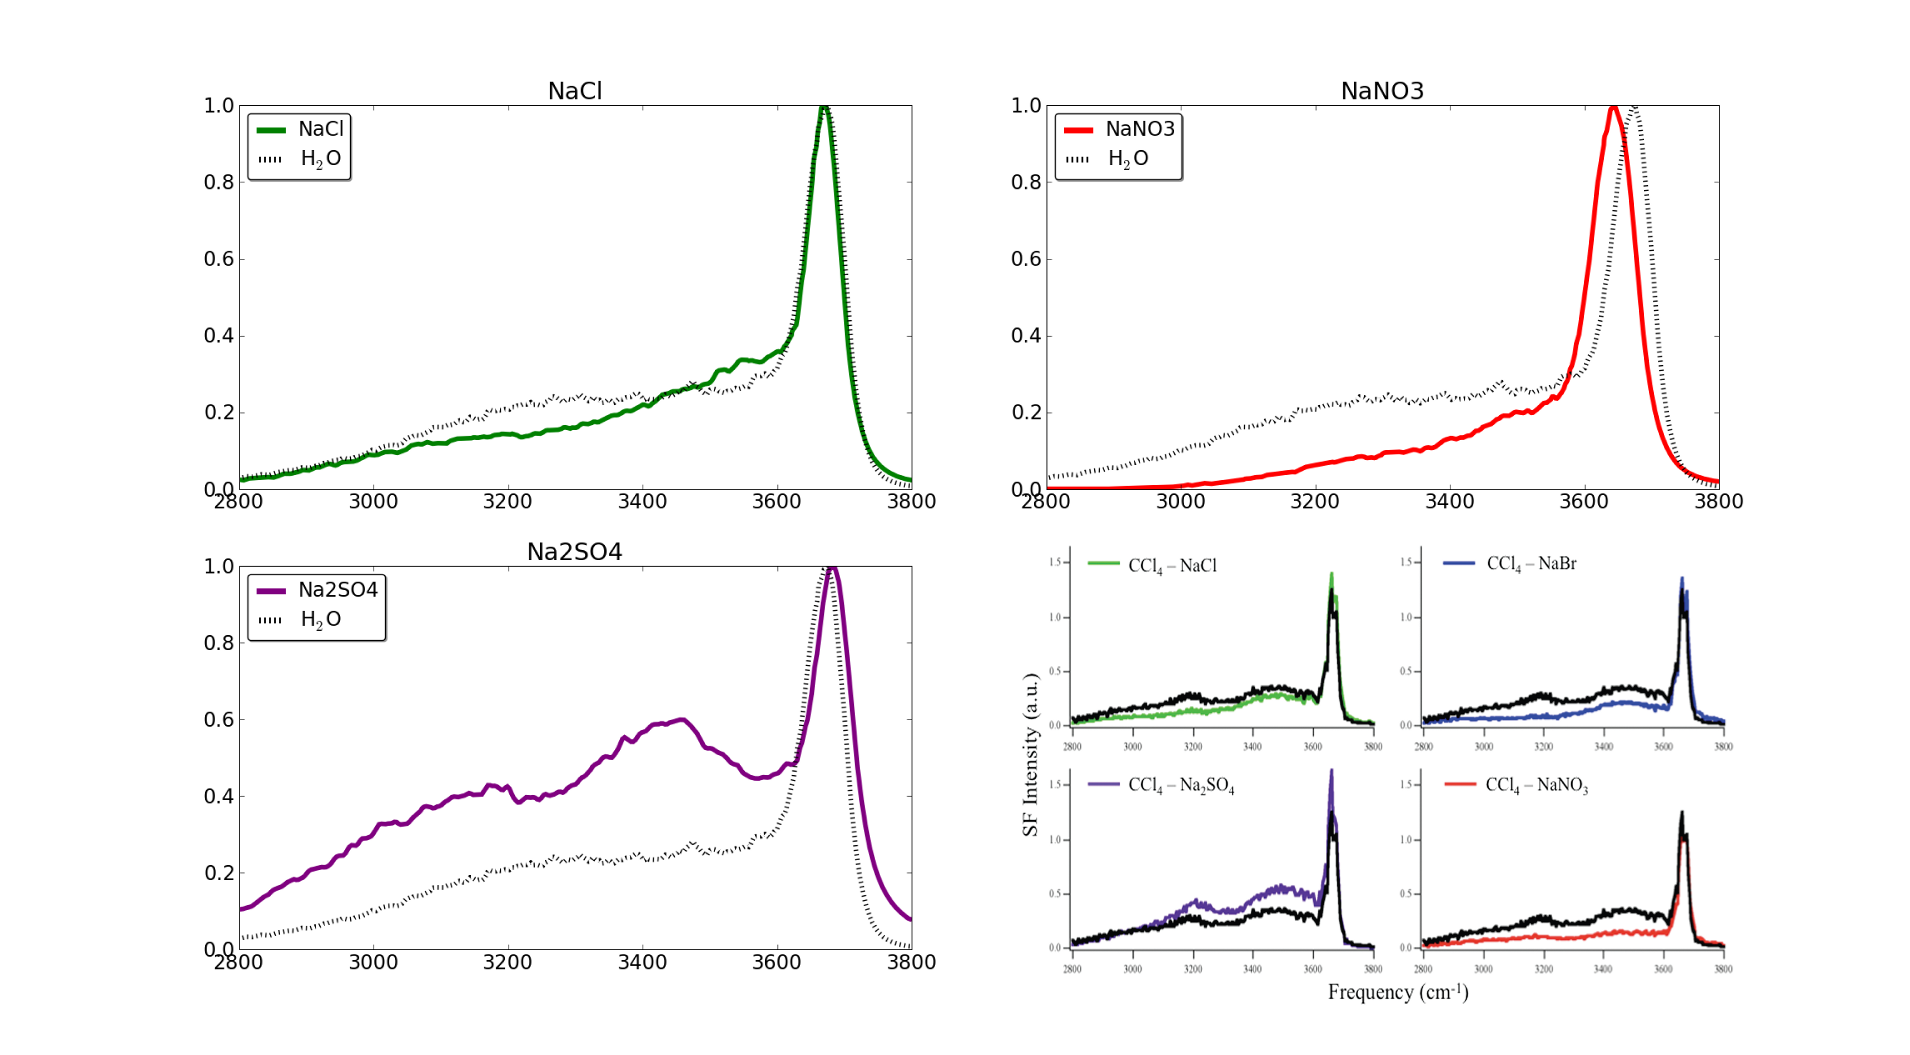
\includegraphics[scale=1.0]{images/sfg-spectra.png}
	\caption{Vibrational SFG spectra of the water-OH stretching region for each interfacial aqueous-salt-\ctc system. The reference \ctcwat interface spectrum (black-dashed line) is provided on each simulated SFG spectrum for reference. Inserts at the top left of each spectrum are reproductions of the experimental spectra ($\chi^{(2)}_{eff}$) from McFearin et al\cite{McFearin2009} including the reference (black) spectrum from that study. SSP polarization is used for all the spectra.}
	\label{fig:sfg-spectra}
\end{center}
\end{figure}

%We have found difficulty in reproducing the lower-frequency peaks near 3200\cm and attribute the slight differences in the lineshape to similar problems reported previously.\cite{Walker2006b} However, 

The reference \ctcwat spectrum reproduces well the lineshape from experiment, but lacks the definition of the two peaks found near 3250 and 3450\cm. These lower-frequency features have been attributed to the different H-bonding species of water that make up the more highly-coordinated, tetrahedral environments found deeper into the interfacial region. The reference \ctcwat lineshape is quite similar to that of the experiment. The salt-solution spectra show an overall drop in signal when \cl and \nit are added and an increase in intensity due to \sul. This suggests that the methods are sound and justified for experimental comparison in this study.

%monovalent ion results
The conclusions drawn from the experiments are that the presence of anions at the interface causes a ``field-screening'' that decreases the innate interfacial field at the \wat-organic interface, and consequently the number of bonded water molecules contributing to the SFG spectrum. Both of the monovalent anions, \cl and \nit, show this effect in their SFG spectra. For both the experiment and these calculations, comparison to the reference \ctcwat spectrum shows that the added presence of the surface-active anions decreases the lower-frequency intensities. Calculations show that \cl affects a notably smaller decrease in the spectral intensities than the \nit system, similar to experiment. This result is most likely due to the higher preference for the surface of the larger, and more polarizable nitrate in the presence of \ctc. The \nit ion is extremely surface active, as seen in the density profile, and should thus cause the greatest ``field-screening'' to waters found deeper in the bulk.

% divalent/sulfate
The larger divalent \sul anion accumulates deeper into the aqueous bulk and exhibits the lowest surface affinity of the ions studied. This is most likely due to the higher charge of the anion that leads to greater solvation. The sulfate provides little or no screening of the interfacial field from the top-most water layer, and more greatly affects the deeper, highly-coordinated waters. The bonding region spanning the lower-frequency features is notably enhanced above the reference spectrum in both experiment and computation. This indicates stronger ordering of deeper interfacial waters, consistent with the anion location.

As concluded in the previous experimental work, the monovalent anions appear to screen the deeper water molecules from the field produced by the phase change at the aqueous-organic interface. This is supported by the MD simulations showing that monovalent ions show a strong surface affinity and interact with surface waters. The large but more highly charged divalent \sul anion experiences stronger solvation and is thus found deeper in the aqueous phase. Deeper anions do not participate as interfacial field screening agents to the same extent as their monovalent counterparts, but act to strongly orient water near the interface, perhaps through the strong field established by the ion double-layering. The distance between the counter-ion density peaks (Table \ref{table:double-layer}) follows the inverse of the trend of SFG signal enhancement. As the ionic double-layer size increases, the SFG signal decreases. Similarly, the smallest double-layer size, that of the \sul system, produces the greatest signal enhancement across the lower frequencies of the water OH-stretching SFG spectrum. Although the water density profiles do not change markedly between the different systems, the orientational profiles do show large variation from the neat \ctcwat system, and some slight variation between the salt-solutions. The two factors that alter the SFG intensity are changes in the number of contributing water bonded species, and a change in orientation of various water bonded species. From the water orientation profiles (Figure \ref{fig:2dhisto}) it is clear that the presence of anions at the \ctcwat interface causes a strong orientation change from the reference \ctcwat system. Thus we find that there appears to be a strong coupling between the presence and size of an ionic double-layer, the subsequent reorientation of surface water molecules, and the resulting SFG signal change.


\section{Conclusions}

The unique environment created by interactions between water and hydrophobic molecules makes ionic adsorption and transport across interfaces possible. Aqueous-hydrophobic surfaces are of prime importance in applications ranging from ion transport, chemical remediation, and catalysis, to chemical synthesis. Complex interfaces between aqueous media and organic phases enhance chemical reactions, and this motivate further research to understand such environments. This study provides an important step in understanding aqueous-organic surfaces by computationally examining simple aqueous salt solutions interfaced with hydrophobic liquid \ctc. Through a combination of simulations and computational analysis, the nature of ionic adsorption and its effect on water hydrogen-bonding, geometry, and orientation at the liquid-liquid boundary is determined.

Analysis of the component density profiles provides a thorough microscopic picture of ionic surface affinity, double-layering, and effect on interfacial size. While the smaller and less polarizable \cl anion behaves at the \ctcwat surface much like at the \airwat one, the larger surface-active anions have altered interactions with water. Density profile analysis shows that the \nit anion exhibits a much greater surface affinity near the organic phase than at an air interface. The orientational analysis of the solutions shows that the salts in each system cause a change to the water orientation at the \ctcwat surface. The orientation profiles show a stratification of water geometries consistent with the emerging picture of a multi-layered surface region with varied geometries and interactions. This reorientation subsequently affects the ionic double-layering and subsurface waters. Such effects are manifested in spectroscopic changes to water's vibrational OH modes. SFG spectra computed in this study build the necessary bridge to our previous SFG work by offering direct comparison of the computational and experimental results. The surface spectroscopic signals are altered relative to the ion-free signal, indicating a change to the water bonding at the interface due to the salts. The divalent \sul anion acts to enhance the surface hydrogen-bonding, while the monovalent ions diminish it. Both the organic phase and the salt anion species in solution act to dramatically alter the geometry and spectroscopy of water's surface. 

We have thus moved toward our goal of further understanding the behavior and impact of ions and a hydrophobic phase on water at liquid-liquid interfaces. The complementing results of both simulation and experiment have strengthened our certainty of some of the underlying surface science of these systems, but challenges still remain. A more complete picture would include knowledge of different cation effects, as well as the changes to the surface by different hydrophobic phases. The ability to analyze these important interfacial environments both theoretically and experimentally now provides us with the tools to better develop our understanding them.

%The \nit density at the interface is enhanced far above the bulk level near an organic phase. 

%Simulations were conducted of the interface between a neat-\wat system, and three aqueous salt systems, and \ctc. By analyzing the density profiles of the water and the various ions in solution we found that both the water and ionic behavior at the liquid-liquid boundary is different than at the air-liquid one. Anions that have been found to be depleted at the air-water interface such as \nit have a strong interfacial affinity at the \ctcwat interface. Similarly, the orientation of water molecules is different at the liquid-liquid interface, and further altered when ions are present in solution. Depending on the ion surface affinity the waters orient to different extents and to different depths, supporting the conclusions of previous simulations and experiment. The field of interface simulation is further exposing the microscopic foundations of the macroscopic experimental results from techniques such as interface-specific spectroscopies. In our work we have connected the simulation results and methods by computing the SFG spectra to further complement previous experimental efforts. Further effort is still needed to provide a fuller understanding of the boundaries of aqueous systems and the effects of salt ions.


\bibliography{WorkCitations}
\bibliographystyle{achemso}

\end{document}
